\chapter{Konzept}
\label{cha:konzept}
Der Aufbau und das Systemdesign des Aktivitäts-Tracking-Frameworks bilden einen zentralen Bestandteil dieser Arbeit. In diesem Kapitel werden die einzelnen Komponenten beschrieben, die für das Tracking von Aktivitätsdaten erforderlich sind. Die praktische Umsetzung des Konzepts erfolgt anschließend in Kapitel \ref{cha:implementierung}.

\section{Systemarchitektur}
Bevor die einzelnen Komponenten im Detail erläutert werden, beschreibt dieser Abschnitt die Zusammenarbeit und die übergeordnete Struktur der Teilbereiche und Systemkomponenten.

\subsection{Komponenten und Aufbau}

\subsubsection{Teilbereiche und Komponenten}
\label{sec:system_design}
Das Tracking-Framework besteht aus sechs Teilbereichen, die gemeinsam den gesamten Funktionsumfang des Systems abdecken.

\begin{itemize}
    \item Systemkonfiguration
    \item Trackingkonfiguration
    \item Daten- und Aktionsermittlung
    \item Filterung und Extraktion
    \item Vermittlung und Ablaufsteuerung
    \item Datenaustausch und Zwischenspeicherung
\end{itemize}

Im Rahmen der Implementierung (siehe Kapitel \ref{cha:implementierung}) wurden diese Teilbereiche in eigenständige Komponenten unterteilt, sodass alle Aufgaben aus diesen Bereichen berücksichtigt werden. Bestimmte Teilbereiche, wie beispielsweise der Datenaustausch und die Zwischenspeicherung, wurden dabei auf mehrere Komponenten verteilt.

\subsubsection{Struktur der Komponenten}
Abbildung \ref{fig:system_design_components} zeigt, wie die einzelnen Komponenten im System zusammenarbeiten. Das zentrale Element bildet der {Tracking-Manager}, über den alle Komponenten miteinander verbunden sind. Jede Komponente verfügt über eine klar definierte Schnittstelle, die den Zugriff ermöglicht. Nur der Tracking-Manager kennt die einzelnen Komponenten, während diese untereinander vollständig entkoppelt und unabhängig voneinander agieren. Die einzige Komponente, die von mehreren Komponenten genutzt wird, ist die Systemkonfiguration. Sie wird vom Tracking-Manager verwaltet und an die jeweiligen Komponenten weitergegeben.

Diese Struktur sorgt für eine hohe Flexibilität. Änderungen, die von der Systemumgebung abhängen, können vorgenommen werden, ohne andere Teile des Frameworks zu beeinflussen. So lässt sich beispielsweise die Art der Datenverarbeitung anpassen, ohne dass der übrige Aufbau geändert werden muss.

\begin{figure}[H]
    \centering
    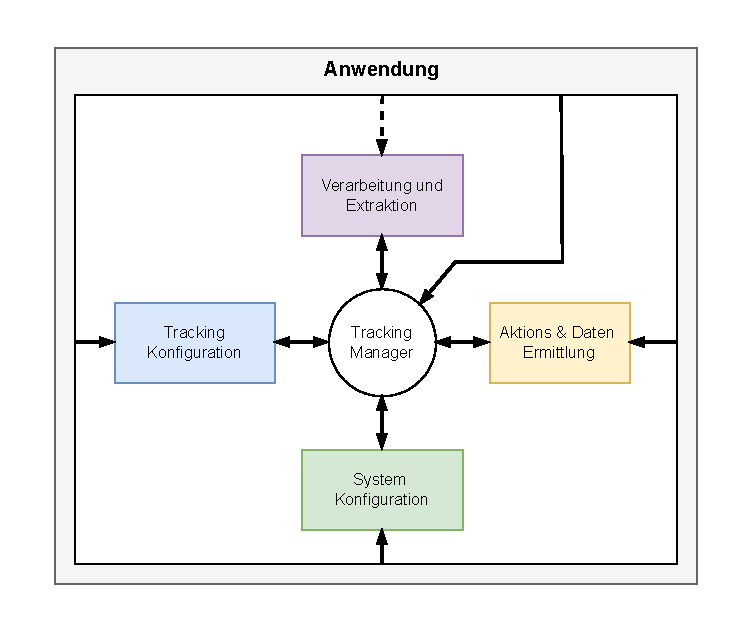
\includegraphics[width=0.8\textwidth]{5_Systemdesign_Components_Tracking}
    \caption{Zusammenhänge der Komponenten im Tracking-Framework.}
    \label{fig:system_design_components}
\end{figure}

Die lose Kopplung besteht nicht nur zwischen den internen Komponenten des Frameworks, sondern auch zwischen der Anwendung und der Datensammlung (siehe Abbildung \ref{fig:system_design_components}). Welche Daten erfasst werden und an welcher Stelle die Erhebung erfolgt, wird vollständig durch das Framework gesteuert.

Die Anwendung selbst muss im Wesentlichen lediglich die erforderlichen Daten über eine definierte Schnittstelle bereitstellen. Dadurch lässt sich das System flexibel in unterschiedlichen Technologien einsetzen, beispielsweise in WPF (siehe Unterabschnitt \ref{subsec:WPF}) oder Windows Forms (siehe Unterabschnitt \ref{subsec:Winforms}).

\subsection{Kommunikation zwischen Komponenten}

\subsubsection{Kommunikationsgrundlage}
Damit ein Informationsaustausch zwischen den Komponenten möglich ist, wird eine gemeinsame Kommunikationsbasis benötigt. Diese Grundlage besteht aus Objekten, die die gemeinsame Sprache für den Datenaustausch definieren.  
Konzeptionell wird zwischen fünf Informationskategorien unterschieden:

\begin{itemize}
    \item \textbf{Trackingaktionen}: Repräsentieren auftretende Ereignisse innerhalb der Anwendung.
    \item \textbf{Trackingdaten}: Umfassen Daten, die auf Basis einer aufgetretenen Aktion erfasst werden.
    \item \textbf{Extraktionsaufgaben}: Beschreiben, welche Informationen aus Trackingaktionen und Trackingdaten ermittelt werden sollen, und stellen Metadaten für die resultierenden Extraktionsdaten bereit.
    \item \textbf{Trackingaufgaben}: Legen fest, welche Daten für die Weiterverarbeitung ermittelt und verarbeitet werden dürfen.
    \item \textbf{Extraktionsdaten}: Enthalten die aus Trackingaktionen und Trackingdaten extrahierten Informationen, die anschließend weiterverarbeitet oder übermittelt werden können.
\end{itemize}

Die einzelnen Kategorien können verschiedene Objekttypen enthalten, die je nach Anwendungsfall unterschiedlich ausgestaltet sind. Diese Objekte bilden einen grundsätzlich unveränderlichen Standard, wobei Extraktionsdaten, Trackingaktionen und Trackingdaten durch benutzerdefinierte Objekte erweitert werden können. Damit die Daten vom Framework verarbeitet werden können, müssen sie, ähnlich wie bei Google Analytics (siehe Unterabschnitt \ref{subsec:google_analytics}), einer festgelegten Struktur entsprechen.

\subsubsection{Datenübertragungswege}
Der Datenaustausch zwischen den Komponenten kann entweder direkt über Rückgabewerte von Funktionen oder über sogenannte Datenkanäle erfolgen.  
Ein Datenkanal ist im Rahmen dieser Arbeit als ein Konstrukt zu verstehen, über das Daten an eine unbekannte oder externe Komponente weitergegeben werden können.  
Durch die Systemkonfiguration (siehe Abschnitt \ref{sec:integration_concept}) kann die Anwendung verschiedene Wege der Veröffentlichung oder des Bezugs von Daten anbieten. Auf diese Weise bleibt das System flexibel gegenüber unterschiedlichen Datenquellen und Zielen.

\subsubsection{Ablauf der Kommunikation}
Der Ablauf der Kommunikation erfolgt über die zuvor beschriebenen Datenobjekte und wird im in Abbildung~\ref{fig:sequence_diagram_communication_components} dargestellten Sequenzdiagramm veranschaulicht.  
Wie dort gezeigt, erzeugt die Anwendung zunächst alle benötigten Komponenten. Die Reihenfolge ergibt sich aus den jeweiligen Abhängigkeiten, wobei die genaue Erstellungsreihenfolge zwischen Datenermittlung (Abschnitt \ref{sec:data_collection_concept}), Verarbeitung (Abschnitt \ref{sec:data_extraction_concept}) und Trackingkonfiguration (Abschnitt \ref{sec:configuration_concept}) nicht entscheidend ist.  

Nach der Erzeugung wird der Tracking-Manager initialisiert. Während dieser Initialisierung wird auch die Systemkonfiguration (siehe Abschnitt \ref{sec:integration_concept}) übergeben. Anschließend initialisiert der Tracking-Manager die Trackingkonfiguration, die wiederum die benötigten Assemblies für die Konfiguration ermittelt. Danach kann der Tracking-Manager die Aufgaben für das Tracking anfordern. Diese Aufgaben werden bei der Initialisierung der Komponenten für Datenermittlung sowie für Verarbeitung und Extraktion berücksichtigt.

Nach Abschluss der Initialisierung kann die Anwendung sogenannte Data Provider registrieren. Dabei entscheidet die Komponente zur Datenermittlung, ob ein Provider einen entsprechenden Datenkanal zur Übertragung von Daten erhält. Über diesen Kanal können sowohl Aktivitätsdaten als auch nachgelieferte Daten gesendet werden.

Die übergebenen Daten werden anschließend in der Extraktionskomponente asynchron zur Anwendung empfangen und weiterverarbeitet.  

Wenn die Anwendung das Ausliefern der Daten anstößt, fordert der Tracking-Manager die Extraktionsdaten an und übergibt sie über den in der Systemkonfiguration bereitgestellten Datenkanal an die entsprechende Zielkomponente.

\begin{figure}[H]
    \centering
    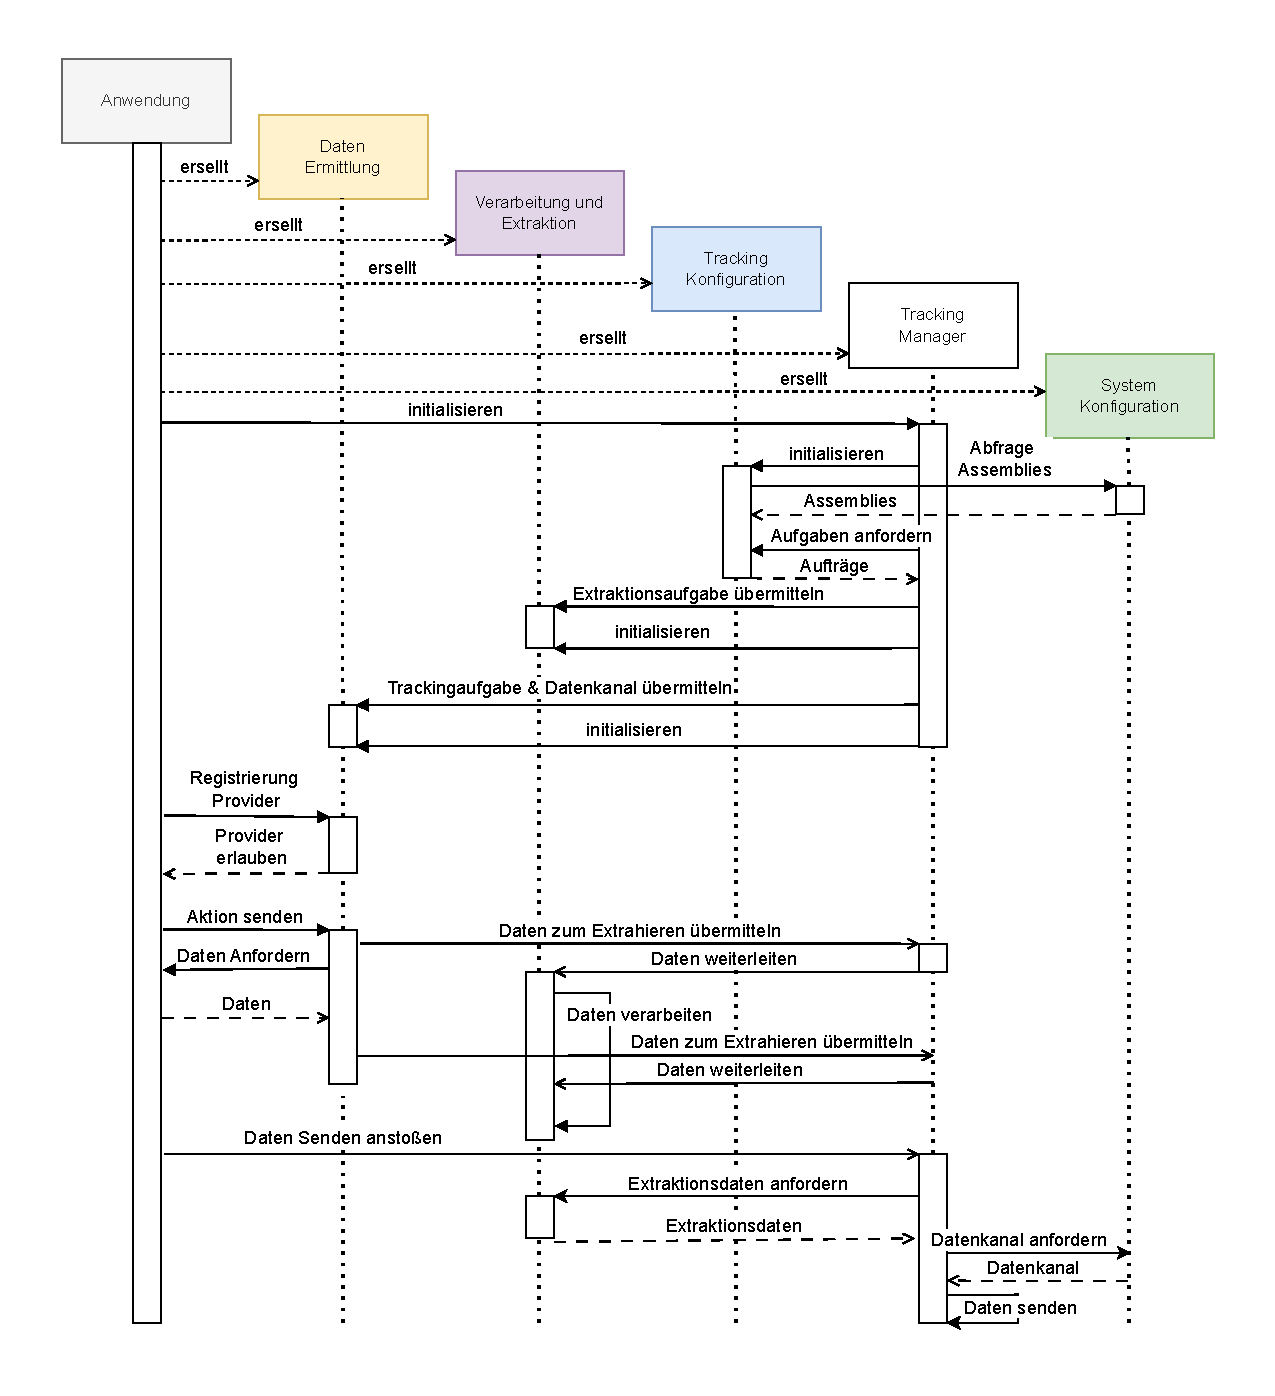
\includegraphics[width=1.07\textwidth]{5_Sequence_Diagram_Components_Communication}
    \caption{Ablauf der Kommunikation zwischen den Komponenten.}
    \label{fig:sequence_diagram_communication_components}
\end{figure}

\section{Tracking-Konfiguration}
\label{sec:configuration_concept}
Wie bei Google Analytics (siehe Unterabschnitt \ref{subsec:google_analytics}) und OpenTelemetry (siehe Unterabschnitt \ref{subsec:open_telemetry}) verfügt auch dieses Framework über eine Konfiguration, in der festgelegt wird, welche Daten getrackt werden sollen. Für das hier vorgestellte Framework ist eine hybride Lösung vorgesehen, die sowohl Online-Konfigurationen, wie bei Google Analytics, als auch Code-basierte Konfigurationen, wie bei OpenTelemetry, ermöglicht. In dieser Arbeit wird jedoch ausschließlich die zweite Variante konzipiert und umgesetzt.

\subsection{Aufbau der Konfigurationskomponente}
Der Aufbau der Konfigurationskomponente ist in Abbildung \ref{fig:configuration_component} dargestellt. Diese Komponente besteht aus einem Manager, der sowohl für die Initialisierung als auch für die Bereitstellung der Aufgaben verantwortlich ist. Der Manager agiert dabei als Slave des Hauptmanagers.

Das Erstellen der Konfiguration erfolgt durch sogenannte Configuration Builder, die zuvor über eine Fluent API \footnote{Unter einer Fluent API oder auch einem Fluent Interface \cite{Fowler2005FluentInterface} versteht man eine Methodik des Method-Chaining, bei der Konfigurationen in einer flüssigen, satzähnlichen Syntax formuliert werden können.} definiert werden. Optional soll die Komponente so erweitert werden können, dass künftig auch ein Konfigurationsserver angebunden werden kann. Im Rahmen dieser Arbeit bleibt dies jedoch unberücksichtigt.

\begin{figure}[H]
    \centering
    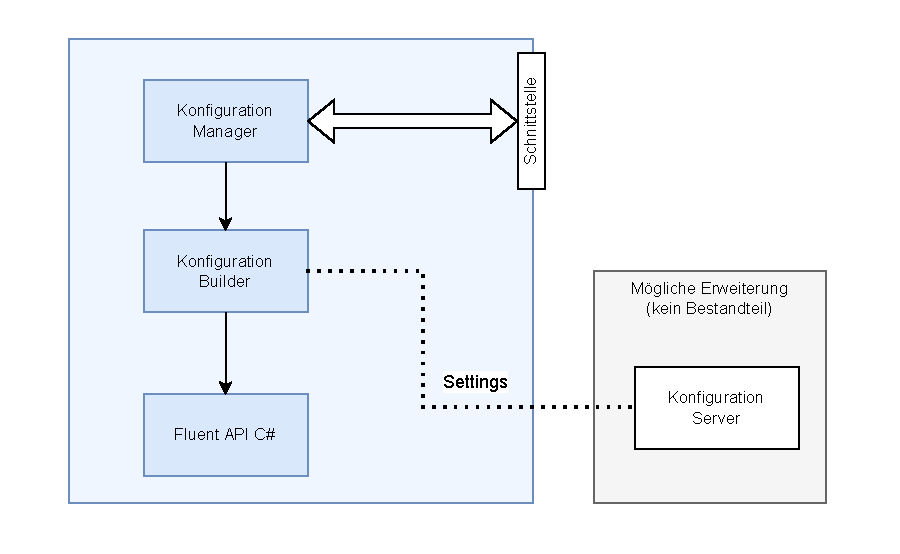
\includegraphics[width=0.8\textwidth]{5_Configuration_Component}
    \caption{Aufbau der Konfigurationskomponente}
    \label{fig:configuration_component}
\end{figure}

\subsection{Konfigurationsmöglichkeiten und Fluent API}

\subsubsection{Kategorien von Informationen}
Um die ursprünglich definierten Fragen (siehe Unterabschnitt \ref{subsec:initial_questions}) beantworten zu können, müssen bestimmte Informationen gesammelt werden. Diese lassen sich in folgende Kategorien einteilen:

\begin{itemize}
    \item \textbf{Metriken:} Zahlenbasierte Daten, wie sie bereits im Zusammenhang mit OpenTelemetry beschrieben wurden. Beispiele hierfür sind die Ladezeit einer Ansicht oder die Anzahl der Öffnungen einer bestimmten Ansicht.
    \item \textbf{Daten:} Informationen, die beispielsweise aus einer Ansicht extrahiert werden können, etwa die Anzahl der Einträge in einer Liste.
    \item \textbf{Nutzung:} Informationen, die Aufschluss über das Nutzungsverhalten der Anwendung geben, beispielsweise wie häufig ein Shortcut in einer bestimmten Ansicht verwendet wird.
    \item \textbf{Workflows:} Informationen, die mit Traces in OpenTelemetry vergleichbar sind und einen Ablauf von aufeinanderfolgenden Aktionen darstellen.
\end{itemize}

\subsubsection{Aufbau der Fluent API}
Die zuvor kategorisierten Daten können weiter beschrieben werden, woraus sich ein Schema ableiten lässt, das für den Aufbau der Fluent API von zentraler Bedeutung ist.\\
\\
$Kontext \rightarrow Kategorie \rightarrow Kategorieoptionen$\\
\\
Daten stammen stets aus einem bestimmten Kontext und gehören zu einer der oben definierten Kategorien. Diese Daten können anschließend durch spezifische Optionen weiter unterteilt werden. Ein vereinfachter Ausschnitt der Fluent API nach diesem Schema wird in Abbildung~\ref{fig:configuration_component_fluent_api} als Syntaxdiagramm dargestellt. Mit der in der Abbildung gezeigten API ist es möglich, das Anfordern von Daten aus einer Ansicht zu konfigurieren.

\begin{figure}[H]
    \centering
    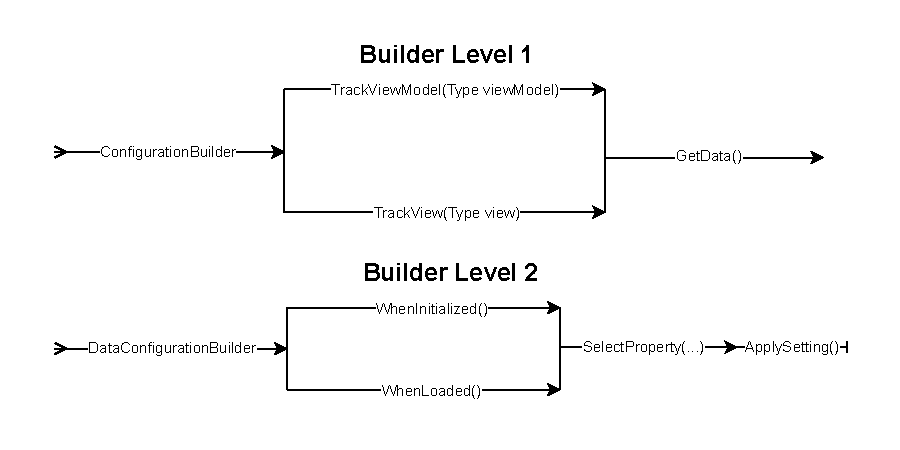
\includegraphics{5_Configuration_Component_Fluent_API}
    \caption{Vereinfachter Ausschnitt der Fluent API für die Tracking-Konfiguration.}
    \label{fig:configuration_component_fluent_api}
\end{figure}

\subsection{Builder und deren Funktionsweise}
Builder \cite{sarcar2004design} sind spezielle Klassen, die konfiguriert werden können und anschließend durch den Aufruf einer Build-Methode entsprechende Objekte erzeugen. Nach der Erzeugung können diese Objekte vom Builder abgerufen werden. Der Director ist die Komponente, die den Erstellungsprozess steuert. Im Kontext dieser Arbeit übernimmt der Manager diese Rolle.

\subsubsection{Bessere Aufgabenteilung durch mehrstufige Builder}
In Abbildung \ref{fig:configuration_component_fluent_api} ist von zwei Builder-Leveln die Rede. Der Grund dafür liegt darin, dass ein einzelner Builder sehr umfangreich und unübersichtlich werden würde. Um die Wartbarkeit und Erweiterbarkeit zu verbessern, werden die Builder daher in mehrere Ebenen unterteilt.  
Der Builder der ersten Ebene ruft die Build Methode der nachfolgenden Ebenen auf und fügt deren Ergebnisse zusammen. Dieses Prinzip folgt dem Composite-Muster \cite{gamma1995design}.

\subsection{Settings und deren Zusammenhang mit Builder}
Aus Sicht der Anwender*innen der API existieren keine Builder direkt. Die Fluent API verwendet stattdessen bestimmte Settings, die am Ende einem Builder hinzugefügt werden. Auf Grundlage dieser Einstellungen kann der Builder anschließend die entsprechenden Objekte erstellen, beispielsweise die Aufgaben zur Datenermittlung (siehe Abschnitt~\ref{sec:data_collection_concept}) und zur Extraktion der Daten (siehe Abschnitt~\ref{sec:data_extraction_concept}).  
Dieser Zusammenhang wird in Abbildung \ref{fig:builder_and_settings_cooperation} dargestellt.

\begin{figure}[H]
    \centering
    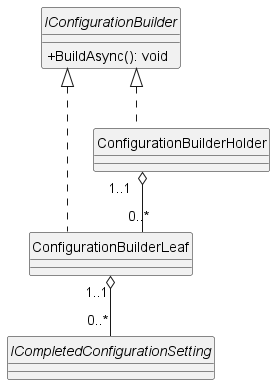
\includegraphics[width=0.4\textwidth]{5_Configuration_Concept_Builder_Class_Diagramm}
    \caption{Klassendiagramm für den Zusammenhang zwischen Builder und Settings.}
    \label{fig:builder_and_settings_cooperation}
\end{figure}

\subsection{Bereitstellen von Einstellungen}
Wie bereits erläutert, werden Einstellungen über eine Fluent-API konfiguriert und einem Builder hinzugefügt. Da Softwaresysteme häufig sehr umfangreich sind, werden sie meist in kleinere Teilprojekte unterteilt. Die in dieser Arbeit behandelte Integration (siehe Kapitel \ref{cha:implementierung}) bezieht sich genau auf ein solches System.

Aus diesem Grund erfolgt die Konfiguration auf Assembly-Basis (siehe Abschnitt \ref{subsec:assemblies}). Konkret bedeutet das, dass pro Assembly mehrere Settings-Provider existieren können, die beim Erstellen einer Konfiguration ausgelesen werden. Diese Provider erhalten eine Starteinstellung (den Einstiegspunkt der Fluent-API) und wenden die entsprechenden Einstellungen automatisch über die API auf einen Builder an.

Diese Provider werden von den Entwickler*innen implementiert, indem die Fluent-API wiederholt auf die jeweilige Starteinstellung angewendet wird. Dabei wird festgelegt, welche Informationen aus dem jeweiligen Teil der Anwendung (der sich in derselben Assembly befinden muss) ermittelt werden sollen.

\section{Daten- und Aktionsermittlung}
\label{sec:data_collection_concept}

\section{Filterung und Extraktion}
\label{sec:data_extraction_concept}

\section{Systemkonfiguration}
\label{sec:integration_concept}


